\documentclass[conference]{IEEEtran}
\usepackage{amsmath,amssymb}
\usepackage{graphicx}
\usepackage{booktabs}
\usepackage{multirow}
\usepackage{xcolor}
\usepackage{algorithm}
\usepackage{algpseudocode}
\usepackage{cite}
\usepackage[hidelinks]{hyperref}

% pending results from the GPU runs; remove before submission
\newcommand{\todo}[1]{\textcolor{red}{[TODO: #1]}}
\graphicspath{{figures/}}

\begin{document}

\title{Why Learned Ecosystems Collapse:\\Energy Leaks, Arms Races and Homeostatic Co-Training}

\author{\IEEEauthorblockN{Mirazul Islam, Fairoze Fatema Alam, Mehejabin Prova, Afnan Zaman Mohammad Sajid and Julkar Naim Shishir}
\IEEEauthorblockA{Department of Computer Science and Engineering\\
United International University, Dhaka, Bangladesh\\
Corresponding author: nnahid929@gmail.com}}

\maketitle

\begin{abstract}
When predators and prey both learn, does their ecosystem survive? We introduce EcoArena, a non-episodic predator--prey world in which grass grows, animals are born, age and die, and nothing ever resets, and we compare five learning methods, from reinforcement learning (PPO) to neuroevolution (GA, ES, NEAT) and a GA-to-PPO hybrid, under an identical reward, network and compute budget. Across 875 test worlds, learning breaks the ecosystem: random animals keep both species alive in 92\% of worlds, ES in 77\%, PPO in 22\% and NEAT in none. Every collapse is the predators dying out, and they die surrounded by prey: a median of 500--570 prey are still alive when the last predator dies. We trace this to two mechanisms. First, an \emph{energy leak}: the net energy a predator gains per step predicts extinction (rank correlation $-0.89$ over 27 trained brains), and evolutionary methods leak because the energy saved by efficient movement is only a quarter of the selection noise in their fitness window. Second, an \emph{arms race the prey win}: slowing prey learning stabilises the ecosystem (ES survives in 100\% of worlds), while slowing predator learning destroys it. Cross-play shows that learned prey of one method starve every other method's predators, and the training objective forms an intransitive game. Both mechanisms are repairable: weighting the movement cost in training turns GA's predators energy-positive and raises its survival from 4\% to 80\%, and a longer discount raises PPO's survival in harsh worlds from 0--4\% to 52--64\%, whereas a shared ecosystem-health reward does not help. Homeostatic Co-Training, a new rule that pauses a species' learning while the other species is rare, gives a smaller gain (ES from 73\% to 87\% of worlds) and cannot repair an energy leak. \todo{E1 GA window.}
\end{abstract}

\begin{IEEEkeywords}
multi-agent learning, neuroevolution, reinforcement learning, predator--prey dynamics, artificial life, benchmark
\end{IEEEkeywords}

% ===================================================================================================
\section{Introduction}

Most learning benchmarks give an agent a task, score it, reset the world and repeat. Ecosystems work differently: many agents act at once, they are born and die, the world never resets, and what is good for one animal can be fatal for its species. A predator that catches everything it sees is an excellent hunter for a while, then starves. Whether learning agents can build a world that \emph{lasts} is a question that episodic benchmarks cannot ask.

We study it in EcoArena, a continuous predator--prey world with grass, refuges, energy, births and deaths, run in parallel on a GPU. We ask two questions at two levels. At the agent level: how well do learned prey avoid predators and learned predators catch prey? At the ecosystem level: when one method controls \emph{both} species, do both species survive?

We compare five methods spanning the two main families for training neural policies: proximal policy optimisation (PPO)~\cite{schulman2017ppo}, a deep genetic algorithm (GA)~\cite{such2017}, OpenAI evolution strategies (ES)~\cite{salimans2017}, NEAT~\cite{stanley2002}, and a hybrid that hands a GA champion to PPO. All share one reward, one network size and one compute budget, measured in world-steps.

The headline result is negative and robust: learning breaks the ecosystem. The rest of the paper explains why. Our contributions are:
\begin{enumerate}
  \item \textbf{EcoArena}, a non-episodic, GPU-batched predator--prey benchmark with a fair-comparison protocol, five scenarios, survival analysis and a browser version that reproduces the simulator step for step.
  \item \textbf{A benchmark} of RL and neuroevolution trained on both species at once, showing that every collapse is predator extinction amid abundant prey, and that training silently hides these collapses.
  \item \textbf{The energy-leak law}: a predator's net energy per step predicts extinction, and evolutionary methods leak energy because a small per-step cost is buried in their fitness noise.
  \item \textbf{Causal evidence for an arms race} won by the prey, from learning-speed interventions and a cross-play tournament analysed with Nash equilibria and $\alpha$-Rank~\cite{omidshafiei2019}.
  \item \textbf{Fixes that work and one that does not}: energy-cost weighting rescues GA (4\% to 80\% survival), a longer PPO horizon rescues PPO in harsh worlds, a shared ecosystem reward fails; and \textbf{Homeostatic Co-Training}, a rule that couples each species' learning to the other's population; it helps ES and PPO modestly and shows that an energy leak cannot be fixed by balancing learning.
\end{enumerate}

% ===================================================================================================
\section{Related Work}

\textbf{Artificial ecologies.} Simulated ecosystems with evolving agents have a long history in artificial life, from Tierra~\cite{ray1991} to PolyWorld~\cite{yaeger1994}. Classical population ecology describes predator--prey cycles with the Lotka--Volterra equations~\cite{lotka1920,volterra1926}.

\textbf{Learning in predator--prey worlds.} Multi-agent RL has used predator--prey tasks mostly as episodic cooperation benchmarks~\cite{lowe2017}. Closer to us, Yang et al.~\cite{yang2018} observed Lotka--Volterra-like dynamics among a million RL agents, Yamada et al.~\cite{yamada2020} studied emergent behaviour in a large-scale predator--prey ecosystem trained with deep RL, Park et al.~\cite{park2021} co-evolved predator and prey RL agents, and Ritz et al.~\cite{ritz2021} found that predators can learn to sustain their prey through emergent cooperation. Each of these uses a single learning method. None compares learning families under a controlled protocol, or tests why ecosystems fail.

\textbf{Social dilemmas.} Over-exploiting a shared resource is a tragedy of the commons~\cite{hardin1968}, studied in multi-agent RL through sequential social dilemmas~\cite{leibo2017,perolat2017}. Ecology frames the predator's version as \emph{prudent predation}~\cite{slobodkin1968} and asks whether restraint can evolve under individual or multilevel selection~\cite{traulsen2006}. The \emph{life--dinner principle}~\cite{dawkins1979} predicts that prey, which lose their lives rather than a meal, win evolutionary arms races.

\textbf{RL versus neuroevolution and multi-agent evaluation.} Deep GA and ES have been shown to be competitive with gradient-based RL~\cite{such2017,salimans2017}, but on single-agent episodic tasks. For evaluating populations of agents, $\alpha$-Rank~\cite{omidshafiei2019} and game-theoretic analyses~\cite{balduzzi2018} handle intransitive interactions that a single score hides. We bring these tools to learned ecosystems.

% ===================================================================================================
\section{The EcoArena Environment}

\textbf{World.} A $200\times200$ toroidal plane holds a $100\times100$ grid of grass that regrows logistically (rate 0.02 per step). Forty-eight circular refuges (radius 6) protect prey from capture, but grass inside them never exceeds 0.35, so hiding forever starves. The benchmark world starts with about 600 prey and 120 predators.

\textbf{Energy.} Every animal holds 0--100 energy. Prey gain energy by grazing (up to 2 per step); predators gain 35 per catch. Living costs 0.10 (prey) or 0.15 (predators) per step, and moving costs an extra $c\,u^2$ per step, where $u\in[-1,1]$ is thrust and $c=0.10$ or $0.15$. Speed persists between steps, so an animal can cruise at full speed with almost no thrust. Animals above an energy threshold breed after a cooldown and hand energy to the child; they die of starvation, of age (1,500 steps) or by being eaten.

\textbf{Hunting.} A predator within 1.5 units of an exposed prey lunges; half of the lunges succeed. A miss stuns it for 40 steps, a catch makes it digest for 60, and a predator cannot breed with more than two others within 15 units. These rules were added until hand-coded animals passed a survival gate: both species alive for 10,000 steps in at least 4 of 5 worlds.

\textbf{Perception and action.} Each animal sees through a cone (prey 240$^\circ$, range 20; predators 120$^\circ$, range 12) split into 16 sectors, each giving the distance and type of the nearest object; with 6 self features this gives 102 inputs. The action is turn and thrust in $[-1,1]$.

\textbf{Scenarios.} Policies are trained on S1 and tested on S1 and four unseen variations: S2 grass regrows at half speed, S3 prey are 30\% faster, S4 both species start at twice the number, and S5 predators start at twice the number.

\textbf{Implementation.} Animals occupy fixed tensor slots per world, so births and deaths never interrupt batched GPU simulation. All randomness is a counter-based hash of (seed, step, stream, world, slot), which lets a TypeScript port reproduce the Python world exactly, as verified by an automated parity test. The browser demo is public.\todo{URL}

% ===================================================================================================
\section{Learners and Protocol}

\textbf{Shared reward.} Every method optimises the same per-step reward for both species: $r_t = \Delta e_t/100 + e^{\text{child}}_t/100 - \mathbb{1}[\text{died}]$, where $\Delta e$ is the energy change and the middle term refunds energy given to newborns, so breeding is neutral. An early version gave PPO a $+1$ birth bonus that evolution could not use; removing it reversed several conclusions, so no method receives it.

\textbf{Methods.} All use a $102\to64\to64\to2$ tanh network shared by every animal of a species (NEAT grows its own, up to 48 hidden neurons).
\emph{PPO}~\cite{schulman2017ppo}: rollouts of 64 steps in 4 worlds, GAE~\cite{schulman2016gae} with $\gamma=0.99$, $\lambda=0.95$, clip 0.2, entropy bonus 0.003; masks handle animals born and dying mid-rollout.
\emph{GA}~\cite{such2017}: 50 genomes, 5 elites, Gaussian mutation $\sigma=0.02$.
\emph{ES}~\cite{salimans2017}: 25 antithetic pairs, centred ranks, Adam~\cite{kingma2015}, learning rate 0.01.
\emph{NEAT}~\cite{stanley2002}: speciation targeting 5 species, compiled to dense batched matrices.
\emph{Hybrid}: GA for half the budget, then PPO from the GA champion after a 20-iteration critic warm-up.
Evolution evaluates all genomes \emph{in the same worlds at once}: slot $s$ is controlled by genome $\pi(s \bmod 50)$ for a 128-step generation, so every genome faces the same ecosystem.

\textbf{Budget and evaluation.} Each run trains both species for 150,000 world-steps (4 worlds in parallel). If a species dies out during training, the world is reset, as is standard. Each of 5 training seeds per method is then tested without learning on 5 fresh worlds for 10,000 steps in all five scenarios: 875 test worlds including the random and hand-coded baselines.

\textbf{Metrics and statistics.} A world \emph{survives} if both species are alive at step 10,000. We also report extinction times, catches per 1,000 predator-steps, lifespans and population stability. The unit of analysis is a training seed. We report bootstrap confidence intervals, exact permutation tests between methods, and Kaplan--Meier survival curves~\cite{kaplan1958} with log-rank tests~\cite{mantel1966}.

% ===================================================================================================
\section{Benchmark: Learning Breaks the Ecosystem}

\begin{table}[t]
\centering
\caption{Worlds with both species alive after 10,000 steps (25 per cell).}
\label{tab:survival}
\setlength{\tabcolsep}{4pt}
\begin{tabular}{lrrrrrr}
\toprule
Method & S1 & S2 & S3 & S4 & S5 & All \\
\midrule
Random     & 100 & 60 & 100 & 100 & 100 & \textbf{92} \\
ES         &  80 & 60 &  84 &  80 &  80 & \textbf{77} \\
Hybrid     &  88 & 40 &  20 &  76 &  96 & \textbf{64} \\
Hand-coded & 100 & 100 & 100 &  0 &  20 & \textbf{64} \\
PPO        &  80 &  0 &   0 &   4 &  24 & \textbf{22} \\
GA         &   4 &  0 &   8 &   8 &  28 & \textbf{10} \\
NEAT       &   0 &  0 &   0 &   0 &   0 & \textbf{0} \\
\bottomrule
\end{tabular}
\end{table}

\begin{figure*}[t]
\centering
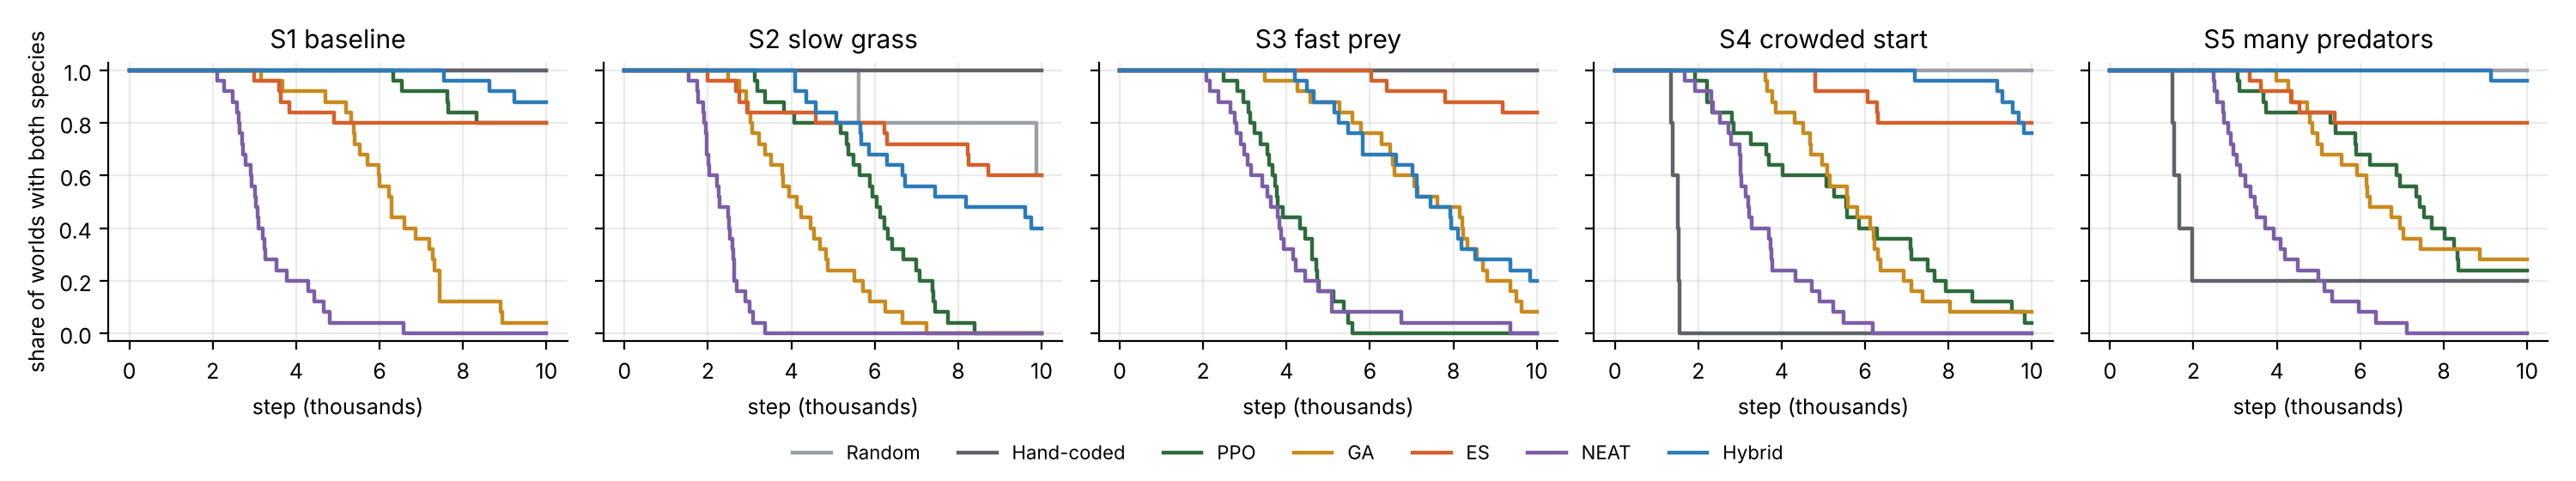
\includegraphics[width=\textwidth]{survival.png}
\caption{Kaplan--Meier curves: share of the 25 test worlds per method still holding both species. Log-rank $p<0.001$ against PPO for most methods in S2--S5.}
\label{fig:survival}
\end{figure*}

Table~\ref{tab:survival} and Fig.~\ref{fig:survival} show the main result. Random animals keep the steadiest ecosystem; of the learners only ES and the hybrid usually survive, and NEAT never does. Three observations shape the rest of the paper.

\textbf{Every collapse is the predators dying out.} Prey never went extinct in any of the 875 worlds.

\textbf{Predators die amid plenty.} When the last predator died, a median of 504--571 prey were still alive for every learned method, close to the starting 660 (the lowest prey count before that was 270--425). Only hand-coded predators over-hunted: their prey fell to 8 before the predators starved. So learned ecosystems do not collapse by over-exploitation. Fig.~\ref{fig:predators} shows two collapse shapes: GA and NEAT predators dwindle from the start, while PPO predators boom, then fade in the harder scenarios.

\begin{figure}[t]
\centering
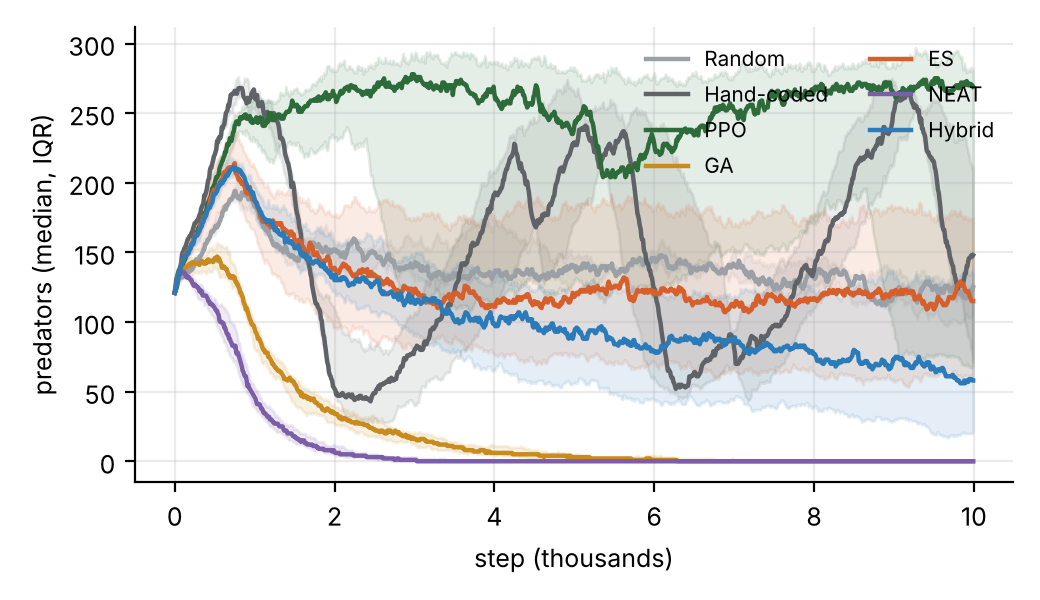
\includegraphics[width=0.95\columnwidth]{predators_S1.png}
\caption{Predators per world in S1 (median of 25 worlds, interquartile band).}
\label{fig:predators}
\end{figure}

\textbf{Training hides collapse.} During training, PPO's worlds collapsed 9--15 times per run and NEAT's 7--12 times; each time the world was silently reset, so no learner was ever penalised for destroying its ecosystem. Outcomes also vary sharply by training seed: ES kept all 25 of its test worlds alive on two seeds and lost 24 of 25 on another.

% ===================================================================================================
\section{Why Learned Ecosystems Collapse}

\subsection{The energy-leak law}

A predator population persists only if, on average, a predator gains more energy than it spends. We measured each brain's movement (thrust$^2$) and combined it with its catch rate (Table~\ref{tab:energy}). PPO predators learned to coast (thrust$^2$ 0.04): they reach top speed and stop pushing. GA and NEAT predators push hard and often reverse thrust (0.56 and 0.73), and lose energy on every step despite catching \emph{more} prey than PPO. Across all 27 trained and baseline brains, net energy and the share of worlds in which predators died out have a rank correlation of $-0.89$ (Fig.~\ref{fig:energy}). The law holds within methods too: the one PPO seed and the one ES seed whose predators collapse in S1 have the thinnest or a negative margin.

\begin{table}[t]
\centering
\caption{Predator energy budget per step (mean over seeds). Cost $=0.15+0.15\,u^2$; income $=$ catches per step $\times35$.}
\label{tab:energy}
\setlength{\tabcolsep}{3.5pt}
\begin{tabular}{lrrrrr}
\toprule
Predators & thrust$^2$ & cost & income & net & died out \\
\midrule
Hand-coded & 0.20 & 0.180 & 0.215 & $+$0.035 & 0\% \\
PPO        & 0.04 & 0.156 & 0.190 & $+$0.034 & 20\% \\
Random     & 0.33 & 0.200 & 0.226 & $+$0.026 & 0\% \\
ES         & 0.18 & 0.177 & 0.195 & $+$0.018 & 20\% \\
Hybrid     & 0.23 & 0.184 & 0.201 & $+$0.017 & 12\% \\
GA         & 0.56 & 0.234 & 0.225 & $-$0.009 & 96\% \\
NEAT       & 0.73 & 0.260 & 0.224 & $-$0.036 & 100\% \\
\bottomrule
\end{tabular}
\end{table}

\begin{figure}[t]
\centering
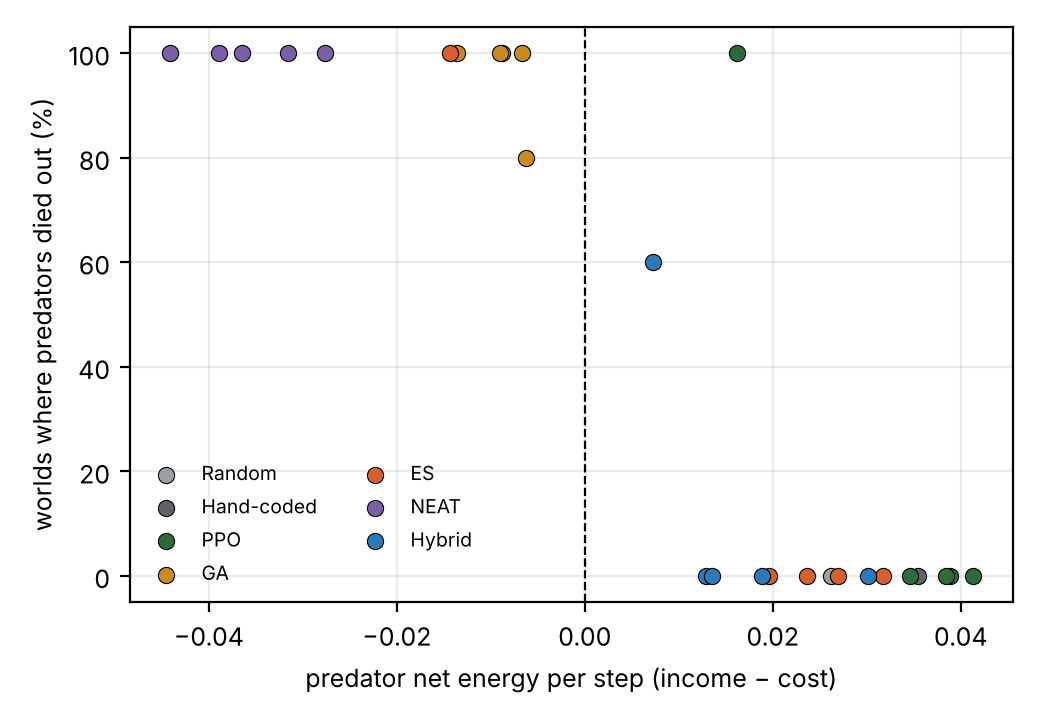
\includegraphics[width=0.85\columnwidth]{energy.png}
\caption{Predator net energy per step against the share of S1 worlds in which predators died out; one point per trained brain.}
\label{fig:energy}
\end{figure}

\textbf{A replacement model.} The law follows from the world rules with no fitted parameter. A predator lives at most $L=1{,}500$ steps, pays $0.15+0.15\,u^2$ per step and gains 35 per catch; each child costs 45 of banked energy, and the 300-step cooldown allows at most five. Treating a brain's catches over a lifetime as Poisson at its measured rate gives the expected number of children per predator,
\begin{equation}
R_0=\mathbb{E}_{k\sim\mathrm{Pois}(cL)}\!\left[\min\!\left(\left\lfloor\tfrac{35k-(0.15+0.15u^2)L}{45}\right\rfloor^{+},\,5\right)\right],
\label{eq:r0}
\end{equation}
and the predators persist only if $R_0\ge1$. The curve $R_0=1$ splits the plane of thrust$^2$ and catch rate into a viable and a doomed region (Fig.~\ref{fig:leakmodel}A): coasting predators need about 4.9 catches per 1,000 steps, predators that push like GA need 7.3, more than any learned predator achieves. Across all 42 brains (benchmark and E4), $R_0$ separates the predator populations that died out from those that survived perfectly (AUC 1.00, Spearman $\rho=-0.88$); the parameter-free threshold $R_0<1$ classifies 83\% correctly, and the errors are all survivors with $0.86\le R_0<1$, because averaging the catch rate ignores that the best hunters father most children.

\begin{figure*}[t]
\centering
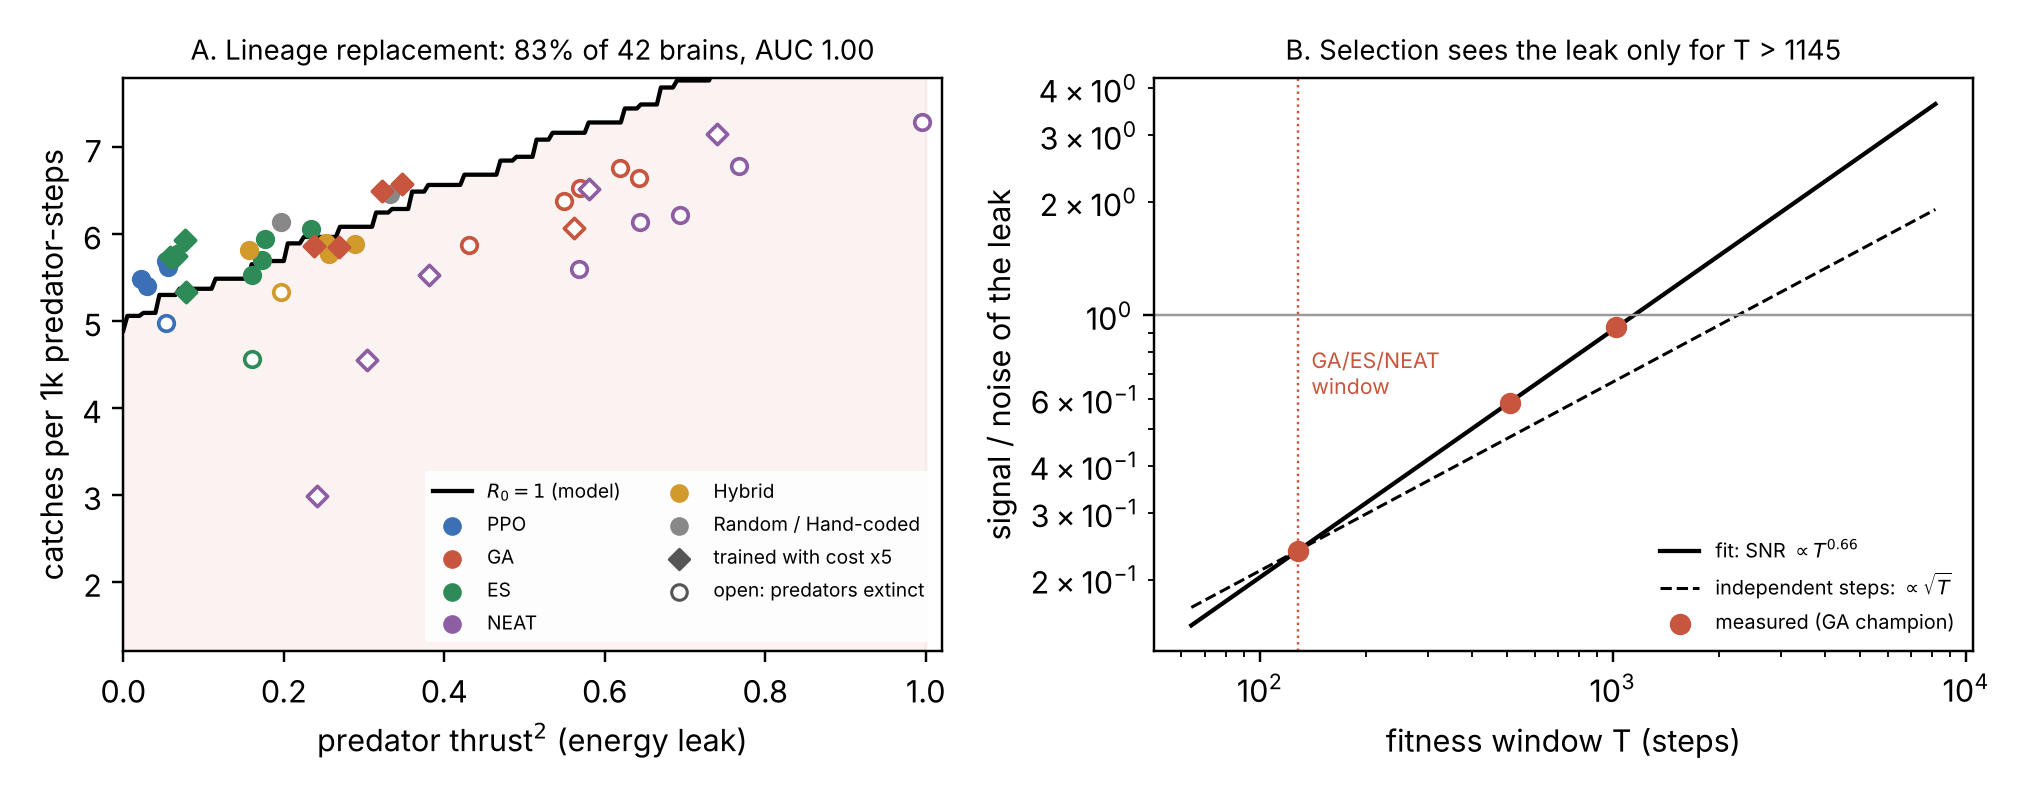
\includegraphics[width=0.92\textwidth]{leak_model.png}
\caption{Analytic model of the energy leak. (A) Each point is one trained brain's predators (open: died out). The line is $R_0=1$ from Eq.~\ref{eq:r0}, using only the world rules; below it a lineage cannot replace itself. (B) How clearly selection sees the energy that coasting saves, against the fitness window. Luck shrinks as $T^{-0.66}$, so the saving only exceeds the luck of catches beyond $T\approx1{,}100$ steps; GA, ES and NEAT rank genomes over 128.}
\label{fig:leakmodel}
\end{figure*}

\subsection{Why evolution leaks}
\label{sec:why}

The energy that coasting saves is small per step: $0.15\times(0.56-0.04)/100\approx0.0008$ reward per predator-step. To test whether selection can see it, we filled all 50 genome slots of GA's shared-world evaluation with the \emph{same} trained predator, so that any fitness difference is pure luck of catches and deaths, and credited half of the slots with exactly the coasting saving. With GA's 128-step window the saving is 0.24 of the luck spread, and the credited half supplies 71\% of the elites (50\% is chance). With 512 and 1,024-step windows the ratio rises to 0.59 and 0.93 and the credited half wins 90--93\% of elite places. The luck spread shrinks as $T^{-0.66}$ (Fig.~\ref{fig:leakmodel}B; independent steps would give $T^{-0.5}$), so the saving outweighs luck only for windows beyond about 1,100 steps, nine times GA's. In a Gaussian selection model the energy trait then receives $d^2/(1+d^2)$ of the selection pressure, where $d$ is the signal-to-luck ratio: 5\% at 128 steps, 26\% at 512 and 47\% at 1,024. Evolution's short fitness window therefore barely sees the cost of wasteful movement, whereas PPO receives it as a per-step reward signal. This predicts that longer windows or a stronger cost signal should repair evolved predators, which we test in Sec.~\ref{sec:fixes}.

\subsection{An arms race the prey win}

\textbf{Cross-play.} We paired every method's prey with every method's predators on S1 (Fig.~\ref{fig:crossplay}). The prey brain matters as much as the predator brain: PPO prey starve the predators of every other method in 72--100\% of worlds, while PPO predators survive against every prey brain in at least 60\% of worlds. GA and NEAT predators die out even against \emph{random} prey (28\% and 92\% of worlds), confirming that their failure is internal (the energy leak), not caused by superior prey.

\begin{figure*}[t]
\centering
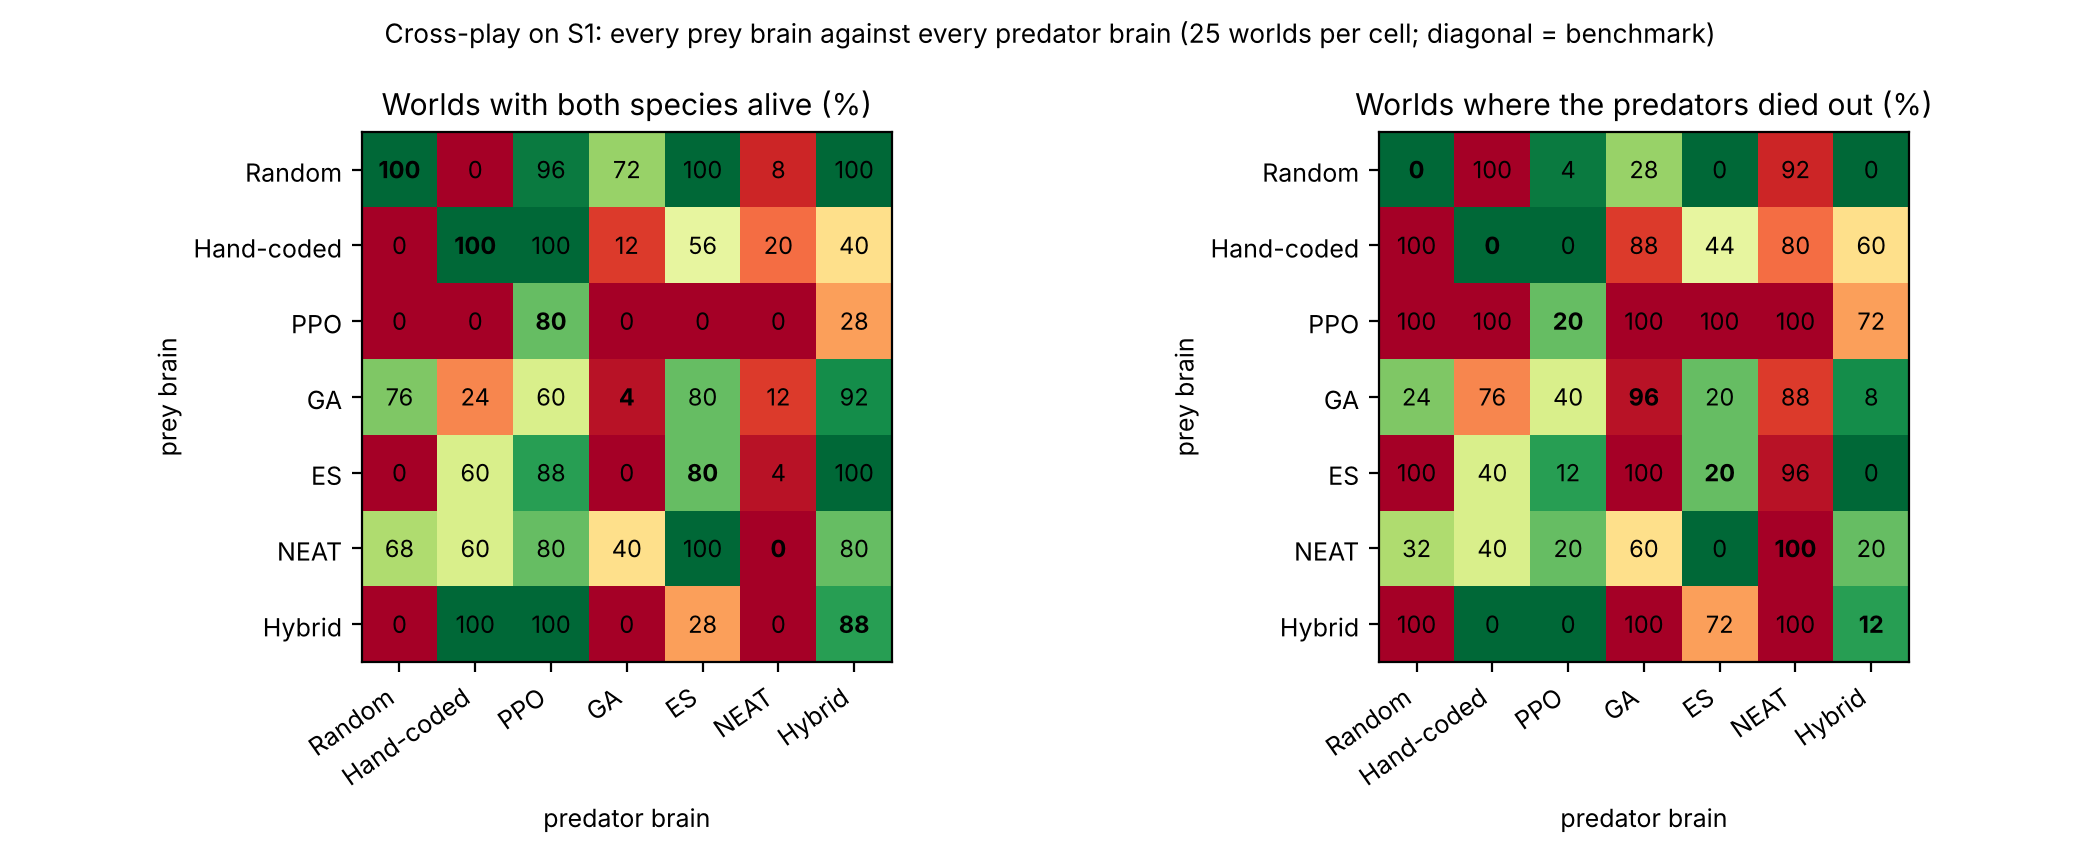
\includegraphics[width=0.85\textwidth]{crossplay.png}
\caption{Cross-play on S1: prey brain (rows) against predator brain (columns), 25 worlds per cell; the diagonal is the benchmark.}
\label{fig:crossplay}
\end{figure*}

\textbf{Learning-speed interventions.} If prey out-learn their predators, slowing prey learning should stabilise the ecosystem and slowing predator learning should destabilise it. We retrained PPO and ES with one species updated only every fourth iteration or generation, or with prey frozen at initialisation (Table~\ref{tab:e3}). Slower prey made ES survive in every test world of all three scenarios, and raised PPO from 0--4\% to 32--40\% in the harder scenarios. Slower predators reduced PPO's S1 survival from 80\% to 0\% ($p=0.048$) and more than doubled its prey's lifespan. Frozen prey fail in the opposite way: untrained prey are eaten out, then predators starve. Balance, not victory for either side, keeps the ecosystem alive. With 5 seeds per condition not every comparison is individually significant, but the direction is consistent across both methods and all scenarios.

\begin{table}[t]
\centering
\caption{Learning-speed interventions (E3): worlds surviving 10,000 steps (\%), 25 per cell.}
\label{tab:e3}
\setlength{\tabcolsep}{4pt}
\begin{tabular}{llrrr}
\toprule
 & Condition & S1 & S2 & S4 \\
\midrule
\multirow{4}{*}{ES}  & baseline           &  80 &  60 &  80 \\
                     & prey learn 4$\times$ slower      & \textbf{100} & \textbf{100} & \textbf{100} \\
                     & predators 4$\times$ slower & 100 &  68 &  84 \\
                     & prey frozen        &  20 &  28 &  20 \\
\midrule
\multirow{4}{*}{PPO} & baseline           &  80 &   0 &   4 \\
                     & prey learn 4$\times$ slower      &  80 & \textbf{40} & \textbf{32} \\
                     & predators 4$\times$ slower &   \textbf{0} &   0 &   0 \\
                     & prey frozen        &   0 &   0 &   0 \\
\bottomrule
\end{tabular}
\end{table}

\textbf{Tournament.} Treating cross-play as a two-population game, we computed equilibria and $\alpha$-Rank~\cite{omidshafiei2019} for two payoffs. Under the \emph{training objective} (each species' own reward) the game has no pure Nash equilibrium and a best-response cycle between PPO/ES prey and PPO/Hybrid predators; its unique equilibrium mixes ES prey (0.94) and PPO predators (0.98). Under \emph{survival} (whether each species persists) the game turns into a coordination game with 11 pure equilibria: viability depends on pairing compatible partners, not on one side winning. What the methods optimise and what keeps the ecosystem alive are different games. $\alpha$-Rank places PPO predators first under both payoffs.

% ===================================================================================================
\section{Preventing Collapse}
\label{sec:fixes}

\textbf{Fixing the energy leak (E4).} If the leak is a signal problem, amplifying the signal should repair it. We retrained GA, NEAT and ES with the movement cost counted five times in the training reward; the world itself is unchanged and evaluation uses the true costs (Table~\ref{tab:fixes}). GA predators cut their thrust$^2$ from 0.56 to 0.35, their net energy turned from $-0.009$ to $+0.014$ per step, and GA's survival rose from 4\% to 80\% in S1 (0\% to 60\% in S2, 8\% to 76\% in S4). The one GA seed whose net energy stayed negative ($-0.022$) is the one seed that still collapsed. ES predators became more economical too (thrust$^2$ 0.07, net $+0.039$, survival 100\% in S1 and 92\% in S2). NEAT is the instructive exception: its predators also cut thrust (0.73 to 0.45) but lost catches (income 0.224 to 0.187), so their net energy stayed negative and they still died out. The energy-leak law held in every case. \todo{E1: GA with a 512-step fitness window and its equal-compute control.}

\begin{table}[t]
\centering
\caption{Fixes: worlds surviving 10,000 steps (\%) and predator net energy per step (S1). 25 worlds per cell.}
\label{tab:fixes}
\setlength{\tabcolsep}{3.2pt}
\begin{tabular}{lrrrr}
\toprule
Condition & S1 & S2 & S4 & net energy \\
\midrule
GA                         &  4 &  0 &  8 & $-$0.009 \\
GA, cost $\times$5         & \textbf{80} & \textbf{60} & \textbf{76} & $+$0.014 \\
ES                         & 80 & 60 & 80 & $+$0.018 \\
ES, cost $\times$5         & \textbf{100} & \textbf{92} & 72 & $+$0.039 \\
NEAT                       &  0 &  0 &  0 & $-$0.036 \\
NEAT, cost $\times$5       &  4 &  0 &  8 & $-$0.030 \\
\midrule
PPO ($\gamma=0.99$)        & 80 &  0 &  4 & $+$0.034 \\
PPO, $\gamma=0.995$        & 88 & 56 & 20 & \\
PPO, $\gamma=0.999$        & \textbf{100} & \textbf{64} & \textbf{52} & \\
PPO, eco reward $\lambda=1$ & 100 & 8 & 0 & \\
PPO, eco reward $\lambda=5$ & 88 & 0 & 16 & \\
\bottomrule
\end{tabular}
\end{table}

\textbf{Longer horizons help; a shared ecosystem reward does not.} PPO's discount $\gamma=0.99$ looks about 100 steps ahead, while collapse unfolds over thousands. Raising it to $\gamma=0.999$ kept every S1 world alive and raised survival from 0\% to 64\% in S2 and from 4\% to 52\% in S4 (Table~\ref{tab:fixes}). By contrast, adding a shared reward for ecosystem health, $\frac{\lambda}{1000}\sqrt{h_\text{prey}h_\text{pred}}$ per animal-step with $h$ the population relative to its start, did not help in the harsh scenarios at either strength. A reward that every animal in a world receives equally gives no individual a reason to act differently, which is the classic obstacle to prudent predation under individual selection~\cite{slobodkin1968,traulsen2006}. Testing group-level selection directly is left to future work.

\textbf{Homeostatic Co-Training.} The arms race suggests coupling each species' learning to the other's state. Our rule (Algorithm~\ref{alg:hct}) pauses a species' updates whenever the other species falls below a fraction $\tau$ of its starting population, so a winning side cannot keep out-learning a collapsing one. For PPO we also replace the silent reset with an extinction penalty $P$ to every learner in a world where a species dies out. We used $\tau=0.5$ and $P=5$, five seeds each, evaluated on S1, S2 and S4. Pooled over the three scenarios, HCT raised ES from 73\% to 87\% of worlds (S2 from 60\% to 84\%) and PPO from 28\% to 39\% (S1 from 80\% to 100\%, S2 still 0\%), but left GA (4\% to 8\%) and NEAT (0\%) where they were. The gate's log shows why. In GA and NEAT training the predators were rare so often that prey learning was paused for 32--66\% of all generations, yet the predators still starved: freezing the prey cannot repair a predator that spends more than it earns. The extinction penalty alone lifted PPO to 43\%, but combined with HCT it fell to 24\%. None of these differences is significant at five seeds (ES: $p=0.07$, Fisher's exact test treating worlds as independent, which overstates the evidence). HCT is therefore a modest stabiliser where no leak exists; the leak and horizon fixes are the strong ones.

\begin{algorithm}[t]
\caption{Homeostatic Co-Training (one iteration)}
\label{alg:hct}
\begin{algorithmic}[1]
\State collect experience or evaluate genomes for both species
\For{species $s \in \{\text{prey}, \text{predator}\}$}
  \State $o \gets$ the other species; $h_o \gets \bar{N}_o / N_o^{\text{start}}$ (mean over worlds)
  \If{$h_o \ge \tau$} update species $s$ (PPO step or next generation)
  \Else{} keep species $s$ unchanged this iteration
  \EndIf
\EndFor
\If{a species is extinct in a world} give its learners penalty $P$; reset that world \EndIf
\end{algorithmic}
\end{algorithm}

% ===================================================================================================
\subsection{Combining the fixes}
\label{sec:combined}
The fixes act on different causes, so we stacked them: for ES, movement cost $\times5$, prey updated four times less often and Homeostatic Co-Training; for PPO, discount 0.999, slower prey and the extinction penalty (HCT gave PPO little). Ten seeds each, tested on S1, S2 and S4 and scored for skill as well as survival, since a world can be kept alive by animals too weak to matter. Skill pits a brain's predators against the prey of all five benchmark methods, and its prey against their predators; 1.0 is the average benchmark method.

The combined ES keeps both species in 96\% of worlds (95\% CI 93--99; ES alone 73\%) at unchanged skill (0.97 against 0.98). The combined PPO reaches 72\% (65--79; PPO alone 28\%) and keeps most of PPO's edge in skill (1.30 against 1.48). Neither reaches the corner we want, high survival with PPO's skill: the steadiest learner is average at hunting and escaping, and the most skilled still loses a quarter of its worlds.

\section{Sensitivity to Step Size}
\label{sec:hyper}
A fair benchmark must ask whether the ranking is an accident of the settings we chose. We retrained every method with its main step size halved and doubled (PPO learning rate, GA mutation size, ES learning rate, NEAT weight mutation), three seeds each, and tested on S1, S2 and S4 (Table~\ref{tab:hyper}).

\begin{table}[t]
\centering
\caption{Worlds with both species alive (\%) when each method's step size is halved or doubled. 15 worlds per cell (3 seeds $\times$ 5 worlds). The 1$\times$ column is the benchmark's seeds 0--2.}
\label{tab:hyper}
\setlength{\tabcolsep}{4pt}
\begin{tabular}{lccccccccc}
\toprule
 & \multicolumn{3}{c}{0.5$\times$} & \multicolumn{3}{c}{1$\times$} & \multicolumn{3}{c}{2$\times$} \\
\cmidrule(lr){2-4}\cmidrule(lr){5-7}\cmidrule(lr){8-10}
Method & S1 & S2 & S4 & S1 & S2 & S4 & S1 & S2 & S4 \\
\midrule
PPO & 67 & 0 & 0 & 67 & 0 & 7 & 93 & 7 & 0 \\
GA & \textbf{100} & \textbf{73} & \textbf{73} & 7 & 0 & 13 & 0 & 0 & 0 \\
ES & 100 & 100 & 80 & 100 & 67 & 100 & 13 & 0 & 0 \\
NEAT & 47 & 33 & 40 & 0 & 0 & 0 & 0 & 0 & 0 \\
\bottomrule
\end{tabular}
\end{table}

\textbf{For evolution the step size matters a great deal, and it acts through the energy leak.} Halving GA's mutation size lifts it from the worst methods (7\% in S1) to the best (100\%), and NEAT from 0\% to about 40\%; doubling either loses every world. The energy budgets show why. With small mutations, GA predators push with thrust$^2$ 0.21--0.33 and earn more than they spend (net $+0.015$ to $+0.033$ per step); with large ones they push at 0.78--0.89 and lose $-0.022$ to $-0.051$. Large random changes drive the thrust output towards its limits, and a 128-step fitness window cannot see the cost well enough to pull it back (Section~\ref{sec:why}). ES behaves the same way, and PPO, which learns from every step, is barely affected.

The replacement model again predicts the outcome without refitting: on these 18 new brains, the main-world threshold $R_0<0.86$ classifies 17 correctly (AUC 1.00), the one miss being a surviving GA seed at $R_0=0.83$.

This changes how the benchmark should be read. The collapse of GA and NEAT is not a fixed property of evolution but of evolution with mutations too large for its fitness window. The benchmark settings were standard defaults, not tuned for survival, and at those defaults the leak appears. The general lesson is unchanged and sharper: in an ecosystem that never resets, a learner's step size is an ecological parameter.

\section{A Second World: Drag}
\label{sec:drag}
To test whether the findings depend on free coasting, we built a second world in which every animal keeps only 90\% of its speed each step before thrust is added, so speed must be paid for continuously. All rules are otherwise unchanged and the browser port matches it exactly. The hand-coded animals keep both species alive in 5 of 5 worlds for 10,000 steps (about 840 prey and 180 predators), so the world is viable. We retrained all five methods with five seeds each and evaluated them on S1, S2 and S4.

\textbf{Learning breaks this world even more.} Only 2 of 375 learned test worlds kept both species (one ES world each in S1 and S4); random animals, which survived 92\% of the main benchmark, now survive none. Once more every collapse is the predators dying out. The five methods' predators push hard to hold speed (thrust$^2$ 0.31--0.80) yet catch fewer prey than the hand-coded predators, which spend less (0.24) and catch more (6.4 against 3.7--6.2 per 1,000 steps). Movement cost $\times5$ rescues GA only partly here (20\% in S1, 0\% in S2, 32\% in S4): with drag the cheap option is gone, and the economical predators the penalty selects for also catch less.

\textbf{The replacement model predicts the new world without refitting.} We measured thrust and catch rate for the 32 drag-world brains (five methods, the GA cost fix and both baselines) and computed $R_0$ from Eq.~\ref{eq:r0}, keeping the threshold fixed at the value found in the main world ($R_0<0.86$). It classifies all 32 correctly (AUC 1.00); the plain rule $R_0<1$ gets 31 of 32. The test is lopsided, with only two surviving brains (the hand-coded animals at $R_0=1.30$ and one GA seed at $R_0=0.864$, exactly on the threshold), so it confirms the model's ranking more than its exact cut.

\section{EcoPPO: a Learner Built from the Causes}
\label{sec:ecoppo}
The fixes above each target one cause. EcoPPO targets all of them at once and keeps everything else of the benchmark PPO (network, update, budget):
(i) a \emph{lineage reward}, counted in children, that charges every step the surplus an animal must bank to raise one child in its life, so break-even predators are penalised as $R_0<1$ demands;
(ii) \emph{no-reset training}: an extinct or collapsed species (below 10\% of its start) is recolonised by migrants, at least 30 predators, instead of the world restarting, and every learner in that world pays a penalty;
(iii) \emph{automatic balancing}: each species' learning rate shrinks by the square of the ratio of the other species' relative numbers to its own, so only the side that is ahead slows down;
(iv) \emph{many worlds}: training worlds S1, S2 and S4, each with drag 0 and 0.1; and a discount of 0.999.

Reaching this version took three iterations, which we report because each failure is informative. Balancing each species against its opponent's starting count (v1) also slowed the losing side; counting only true extinctions let migrants hide collapse from the learner. With those corrected (v2) the predators still crashed early in training and only some seeds recovered. Freezing the prey for the first quarter of training (a curriculum) made matters worse: when the prey resumed learning, the predators crashed again. What worked was the larger migrant floor alone, which kept enough predators to learn from.

\begin{table}[t]
\centering
\caption{EcoPPO, 10 seeds, worlds with both species alive (\%), 50 per cell. Training saw S1, S2, S4 at drag 0 and 0.1; S3, S5 and drags 0.05 and 0.15 are unseen. Benchmark PPO in brackets (5 seeds).}
\label{tab:ecoppo}
\setlength{\tabcolsep}{4.5pt}
\begin{tabular}{lcccccc}
\toprule
World & S1 & S2 & S3 & S4 & S5 & All \\
\midrule
Drag 0 & 90 (80) & 80 (0) & 70 (0) & 62 (4) & 88 (24) & 78 (22) \\
Drag 0.05$^\ast$ & 96 & 82 & 80 & 72 & 88 & 84 \\
Drag 0.1 & 98 (0) & 42 (0) & 70 (0) & 86 (0) & 100 (0) & 79 (0) \\
Drag 0.15$^\ast$ & 10 & 0 & 4 & 8 & 8 & 6 \\
\bottomrule
\multicolumn{7}{l}{\footnotesize $^\ast$ never seen in training}
\end{tabular}
\end{table}

EcoPPO keeps both species in 78\% of main-world tests against PPO's 22\%, including the two unseen scenarios, and in 79\% of drag worlds, where every benchmark learner kept none. It interpolates to the unseen drag of 0.05 (84\%) but does not extrapolate to 0.15 (6\%), although hand-coded animals survive there in every test: training across worlds widens what a learner can handle, but only to the range it has seen. Its animals stay skilled (1.12 against the benchmark average of 1.0; PPO 1.48, ES 0.98). \todo{ablations, PPO and ES at drag 0.05 and 0.15}

\section{Discussion and Limitations}

Our results point to two separable failure modes. Evolutionary methods with short fitness windows produce energetically wasteful predators that starve whatever their prey do; gradient-based RL produces efficient predators but even more effective prey, and the ecosystem survives only while neither side out-learns the other. Neither failure is visible in the training objective, and both are hidden in standard practice by resetting worlds after extinction. This matches ecological intuition, the life--dinner principle~\cite{dawkins1979} and the difficulty of evolving prudence under individual selection~\cite{slobodkin1968}, but here it is measured, manipulated and quantified.

\textbf{Limitations.} Both worlds share one design (2D, continuous, energy-based), small networks and a fixed budget of 150,000 world-steps; larger budgets may change rankings. Five training seeds limit the power of individual comparisons, and outcomes depend strongly on the seed. The energy budget combines thrust measured over a short window with catch rates from the full evaluation. We did not test group-level selection, which our GPU budget could not cover. \todo{update after E1/E5.}

\section{Conclusion}

Learning agents that each optimise their own energy tend to destroy the ecosystem they live in. In EcoArena this happens through energy leaks in evolved predators and an arms race won by learned prey, and it is hidden by the common practice of resetting after extinction. Making the cost of movement visible to evolution, or lengthening PPO's horizon, keeps far more ecosystems alive; rewarding ecosystem health directly does not. Homeostatic Co-Training adds a modest margin where no leak exists, but no balancing of learning can save predators that spend more energy than they earn. The environment, all runs and the browser demo are open source.\todo{repository URL}

\bibliographystyle{ieeetr}
\bibliography{refs}

\end{document}
